\section{分餐与合餐}
\par
中国与德国存在着诸多文化上的差异,这既是地理因素所决定的,同时也是人文历史发展的影响。现在就让我们从饮食文化角度着手,一探两国的文化差异,体会一番中德两国彼此的异域风情。说到饮食就不得不提及中德两国的用餐礼仪。中国的合餐制与德国的分餐制。就让我们窥一斑而知全豹,从分餐与合餐入手,细细体会中德两国之间文化的魅力。
\par
中华上下五千年,在汹涌的历史长河中,不但伴随着王朝的更替,同时也伴随着人们生活观念的改变。民以食为天,在中国吃饭可是件大事,中国人向来不敢怠慢。在周秦汉晋时期,人们注重分餐的礼仪,十数人席地而坐,在各自的小桌前,静静的等待厨师将分配好的食物端上桌来。期间无论有多么饥饿,大家也要正襟危坐,保持严肃,把嘴巴里的口水咽回到肚子里去。据《史记•孟尝君列传》记载,一个不懂规矩的客人,因为嫌弃自己桌上的饭菜不够可口,在用餐期间向主人大发脾气,但是在看到身份高贵的主人,他桌前的饭菜和自己吃一样时,而羞愧难当。这也正是一人一桌,彼此之间保持一定的距离的用餐制度在中国历史上最生动的一次写真。时光飞逝,在进入唐宋时期后,随着社会生产力的提高,使得用餐制度的改变成为可能。唐朝,这个由李唐文明建立的宏伟帝国,与历史上任何一个朝代都有所不同,它是繁荣的象征,是昌盛的象征,更是和谐与包容的象征。少数名族经河西走廊,过敦煌进山海关,来到长安,这座当时的国际大都市。他们不但带来了人们从未见过的异域特产,更重要的是他们还带来了他们的饮食作息与习俗。他们不知道他们的高桌大椅,很快就会改变这个拥有古老历史的中华民族,在他们的餐桌上掀起一场,影响深远的饮食文化革命。在见识了,这些批头散发的胡人在大桌大椅上,毫无顾忌的吃喝后。唤醒了华夏人民心灵深处,由分向合的,由差异向大一统的强烈渴望。人们不由自主的爱上了这些高大的桌椅。从此高桌椅凳,一家人围桌而食,成了人们社会生活的主流。从富有历史的分餐制到现如今的合餐制,是中华文明的一种转变,也是中国文化的一种体现:⑴亲密关系  圆桌而坐 团团圆圆,是君子温润如玉,互敬互让,关心他人,谦让美德的表现现。也是大一统思想表征,说明了人们期望增加民族的凝聚力和社会的和谐。⑵促进合作  人们在合餐时,促进沟通,相互了解,增加合作。⑶解决争端  解决矛盾增加和谐。⑷多样性选择  食物的多样性,供人们选择,有人喜欢,有人不喜欢,彼此之间不排斥,互相包容。⑸以和为贵,万事通荣 大家在节假日中商议选菜,互相尊敬,包容。

\begin{figure}
\centering
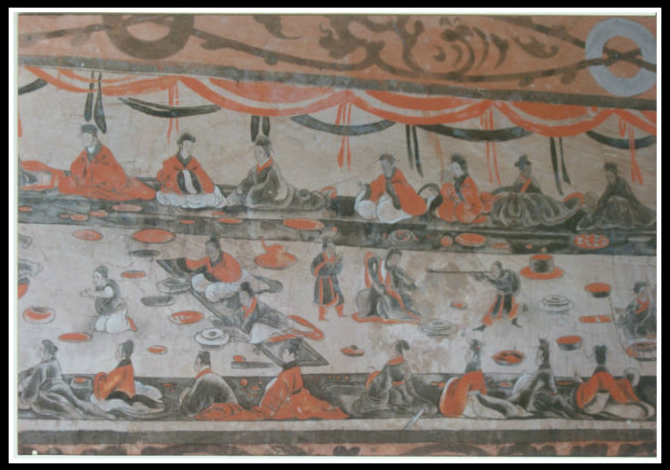
\includegraphics[width=0.6\linewidth]{Essen_in_Han_Dynastie}
\caption{汉朝时期的分桌而食}
\end{figure}

\begin{figure}
\centering
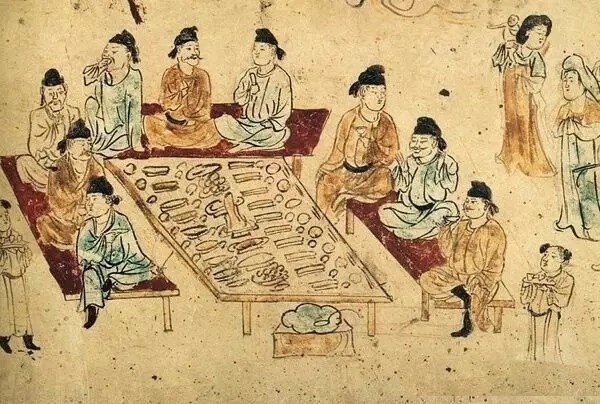
\includegraphics[width=0.45\linewidth]{Essen_in_Tang_Dynastie}
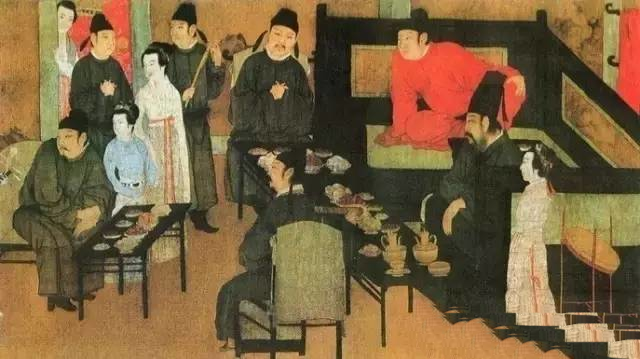
\includegraphics[width=0.45\linewidth]{Essen_in_song_Dynastie}
\caption{唐宋时期的合桌而食\protect\footnote{受北方少数民族影响唐宋时期人们平时宴饮开始围桌合餐。右图为北宋著名的韩熙夜宴图}}
\end{figure}
\par
分餐制在西方一直持续至今。文献记载从文艺复兴时期到维多利亚时代,欧洲贵族由佣人把菜端到桌子上,把大盘食物分到每个人的盘子里。而平民在厨房中吧食物分配好,再端到每个人面前。之所以分餐制能在贵族和平民之间如此流行。主要是因为⑴人们对注重饮食卫生的注重 ⑵曾经肆虐欧洲的黑死病,夺取了无数人们的生命,这种对黑死病的恐惧,深深植根在人们心中。⑶随着第一次与第二次工业革命的到来,极大的促进了社会的生产力,使人们更加富裕,使得在有钱人和贵族的分餐礼仪在中产阶级中流行起来。这样的分餐制也反应了欧洲文化的一种特点:人与人之间互不干扰,各负其责。
\begin{figure}
\centering
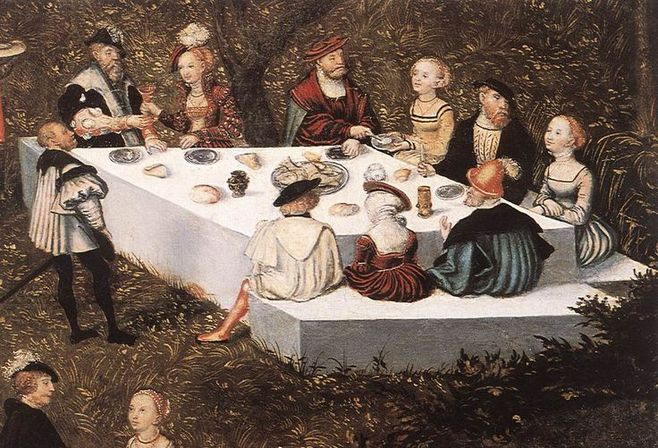
\includegraphics[width=0.45\linewidth]{Essen_in_Deutschland}
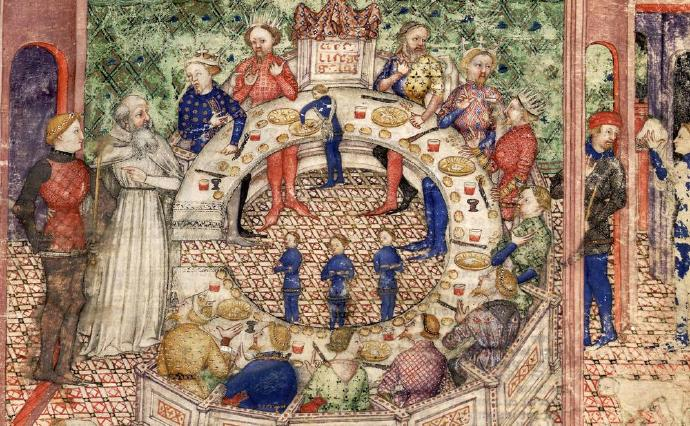
\includegraphics[width=0.45\linewidth]{Essen_in_Deutschland1}
\caption{欧洲人分餐的情形}
\end{figure}

\par
分餐与合餐是中德之间巨大的文化差异。德国:注重个人主义文化,独立自主,尊重隐私,理性分析和他人的利弊得失。而中方:注重集体主义,尊重互敬,爱护和支持关心他人。中国人喜欢给客人加菜,中国人认为这是人和人尊敬谦让的体现。而若是在德国,恐怕会被认为是个人的自由自主被侵犯。同时中国人在一张大桌上吃同一盘菜,难免会越身取食,在经过别人面前时,中国人不认为是不尊重的表现,反而是亲密关系的体现。这是文化中和谐包容的表现。而对于德国人会觉得私人空间被侵犯。因为德国的文化比较注重个人的隐私。
\par
从中德的餐桌文化差异,可以看到两国人民的文化特点。无论是中国还是德国,文化上都没有所谓的优劣,这些文化是中德两个国家的人民的智慧的结晶。他们像夜空中的繁星,点缀着人类文明的浩瀚银河。
